\subsection{Mass Transfer Across Phases}
\label{sec:MT_Phases}
The term, $C_{int}$ in equation \ref{eqn_migration} is, in some sense, not well defined.  The liquid interface can be defined as the monolayer of atoms that are in contact with the gasseous phase, whereas concentration is a volumetric term.  To overcome this difficulty,  we employ the \textit{two-film model} to model the rate of mass transfer across a gas/liquid phase interface.  The figure \ref{twoFilm} shows a phase interface as conceptualized by two-film theory.


\begin{figure}[ht]
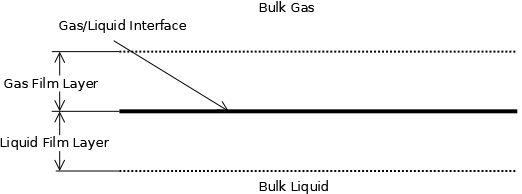
\includegraphics[width=\textwidth,height=\textheight,keepaspectratio]{GFX/twoFilm.png} 
\caption{Illustration of two film theory}
\label{twoFilm}
\end{figure}

The two film model is detailed by Albright. \cite[p. 604]{Albright2008}  In brief, the model partitions space into bulk liquid, liquid film, gas film, and  bulk gas layers.  Between the liquid and gas sfilm layers is a liquid/gas interface.  Each film layer is modeled by Whitman's stagnant film model wherein each film layer is of thickness $x_0$ and is assumed quiescent. [ibid. 602]  The mass transfer process is then governed by diffusion and the mass flux across the film layer is governed by Fick's first law,

\begin{equation}
    J = - D \frac{dC}{dx}, 
\end{equation}
where the diffusion coefficient is the mass diffusion coefficient for a particular solute.  The mass transfer coefficient for a given film layer is defined as,
\begin{equation}
    \label{kmDef}
    k_m = \frac{1}{R_m} = \frac{D}{x_0}.
\end{equation}

In this way, the mass transfer problem can be reduced to a series resistance problem, illustrated in figure \ref{fig:twoResist}
\label{fig:twoResist}
\begin{figure}[ht]
\begin{center}
    

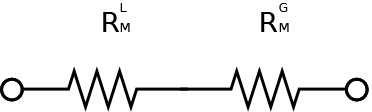
\includegraphics[width=0.5\textwidth,height=0.5\textheight,keepaspectratio]{massTwoResist.png}
\caption{Mass transfer modeled as a two resistance problem}
\end{center}
\end{figure}

According to Perry, the mass diffusion coefficients of gasses are much greater than that of liquids. \cite[sec. 5 p. 48]{Perry2008} Therefore, since ,
\begin{equation}
    D_g >> D_L,
\end{equation}
and, considering equation \ref{kmDef}, it follows,

\begin{equation}
    R_m^g+R_m^L \approx R_m^L,
\end{equation}
and the overall mass transfer coefficient, $K_m \approx 1 / R_m^L$.

We can thus approximate the mass transfer across the phase interface as,

\begin{equation}
    \label{eqn_MT_int}
    J = K_m (C^{B,L}-C^{int,L}).
\end{equation}

We next invoke Henry's law for an ideal gas which states,
\begin{equation}
    \lim_{C\to 0 }  \frac{C ^L}{p^G} = H_i.
\end{equation}
More information on Henry's law is given by Albright. \cite[p. 13]{Albright2008} Equation \ref{eqn_MT_int} can be rewritten as,

\begin{equation}
    J = K_m (C^B-H_i p_i^{F,G}).
\end{equation}
Further, we assume,
\begin{equation}
    p_i^{F,G} \approx p_i^{B,G},
\end{equation}
the partial pressure of the dissolved gas in the gas film layer is approximately equal to the partial pressure of the gas in the bulk; this is justified on the grounds that the diffusion process in gasses is much faster than the diffusion processes in liquid, consider the relative magnitudes of their mass diffusion coefficients.  Thus,

\begin{equation}
    J = K_m (C^B-H_i p_i^{B,G}).
\end{equation}

Invoking the ideal gas law, $p = CRT$, we write

\begin{equation}
    J = K_m (C^{B,L}-H RT C^{B,G}).
\end{equation}

Forms of this equation are ubiquitous in MSR xenon analysis literature.  In the transfer of mass from fuel salt to graphite, the concentration term for the graphite is divided by an effective void fraction term,

\begin{equation}
    J = K_m (C^{B,L}-\frac{H RT}\epsilon{} C^{B,G}),
\end{equation}
so the porosity of the material is accounted for.